\section{Tracker}

\subsection{Inner Detector}
\label{inner_detector}

A cutaway view of the inner detector for ATLAS is shown in \Fig{ATLAS-InnerDetector}.
\begin{figure}[h!tbp]
\centering
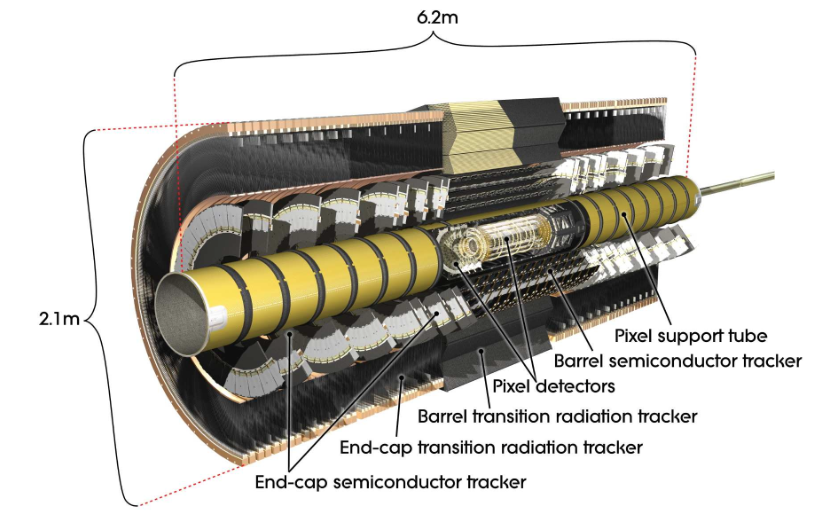
\includegraphics[scale=0.9]{\figpath/ATLAS_inner_detector.png}
\caption{Illustration of the orientation of the subsystems inside the ATLAS Inner Detector~\cite{Aad:2008Jinst}}
\label{ATLAS-InnerDetector}
\end{figure}

\begin{figure}[h!tbp]
\centering
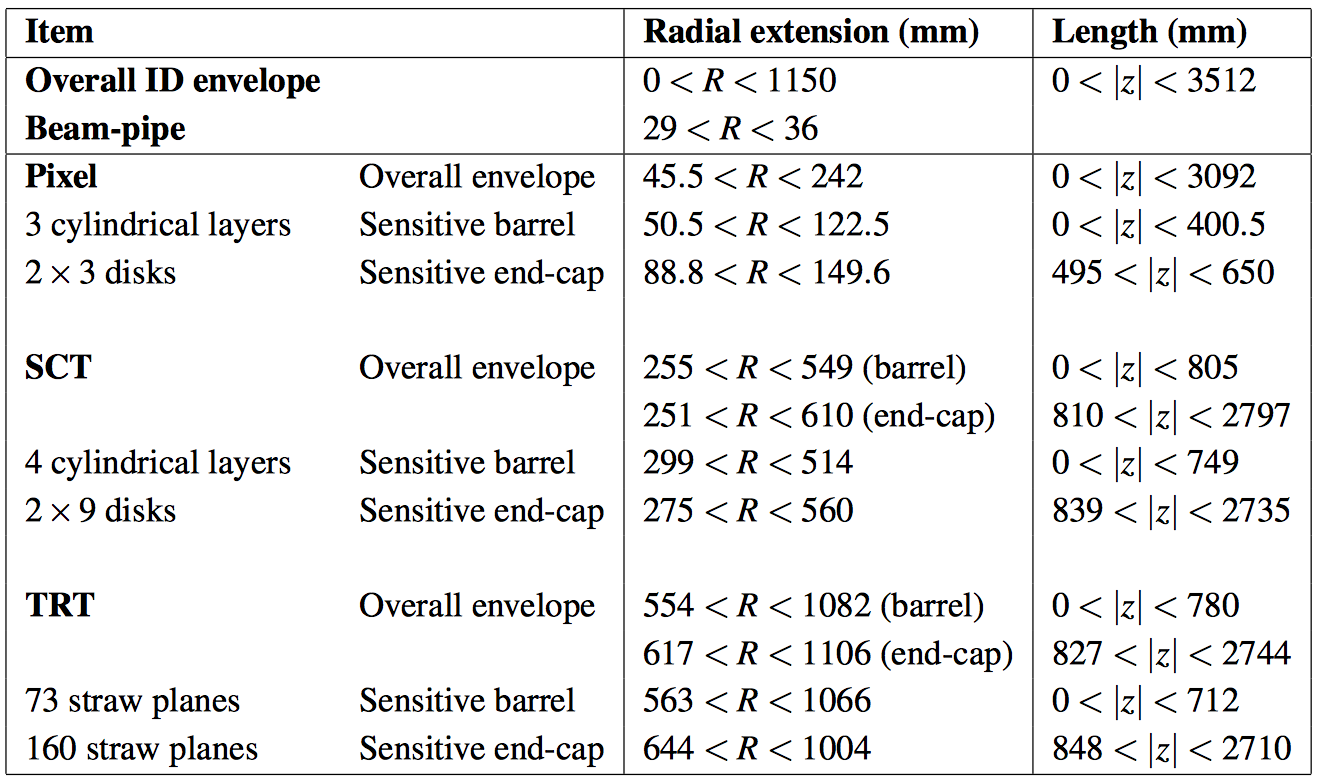
\includegraphics[width = \textwidth]{\figpath/ID_table.png}
\caption{List of the dimensions of the subsystems in the ID~\cite{ATLAS_long}.}
\label{ID-table}
\end{figure}
With approximately 1000 tracks emerging from the interaction point every 25~ns, the ID is divided into three different regions to optimize the pattern recognition and momentum measurement algorithms \cite{ATLAS_long}.  
The pixel detectors have the most precision, so this layer is closest to the interaction point. The pixel detector also has the highest cost, so the next least expensive tracking option is the silicon microstrip trackers (SCTs), at the next farthest region away from the interaction point.  Finally, the Transition Radiation Trackers (TRTs) compose the outermost region of the inner detector.
The ID uses pattern recognition to measure transverse momentum as low as 0.5~GeV, and provides electron identification for $|\eta| < 2.0$ for energies up to 150~GeV \cite{ATLAS_long}. Displaced multi-particle vertexes can be resolved by the pixel detector and help identify long-lived B-hadrons.

\begin{figure}[h!tbp]
\centering
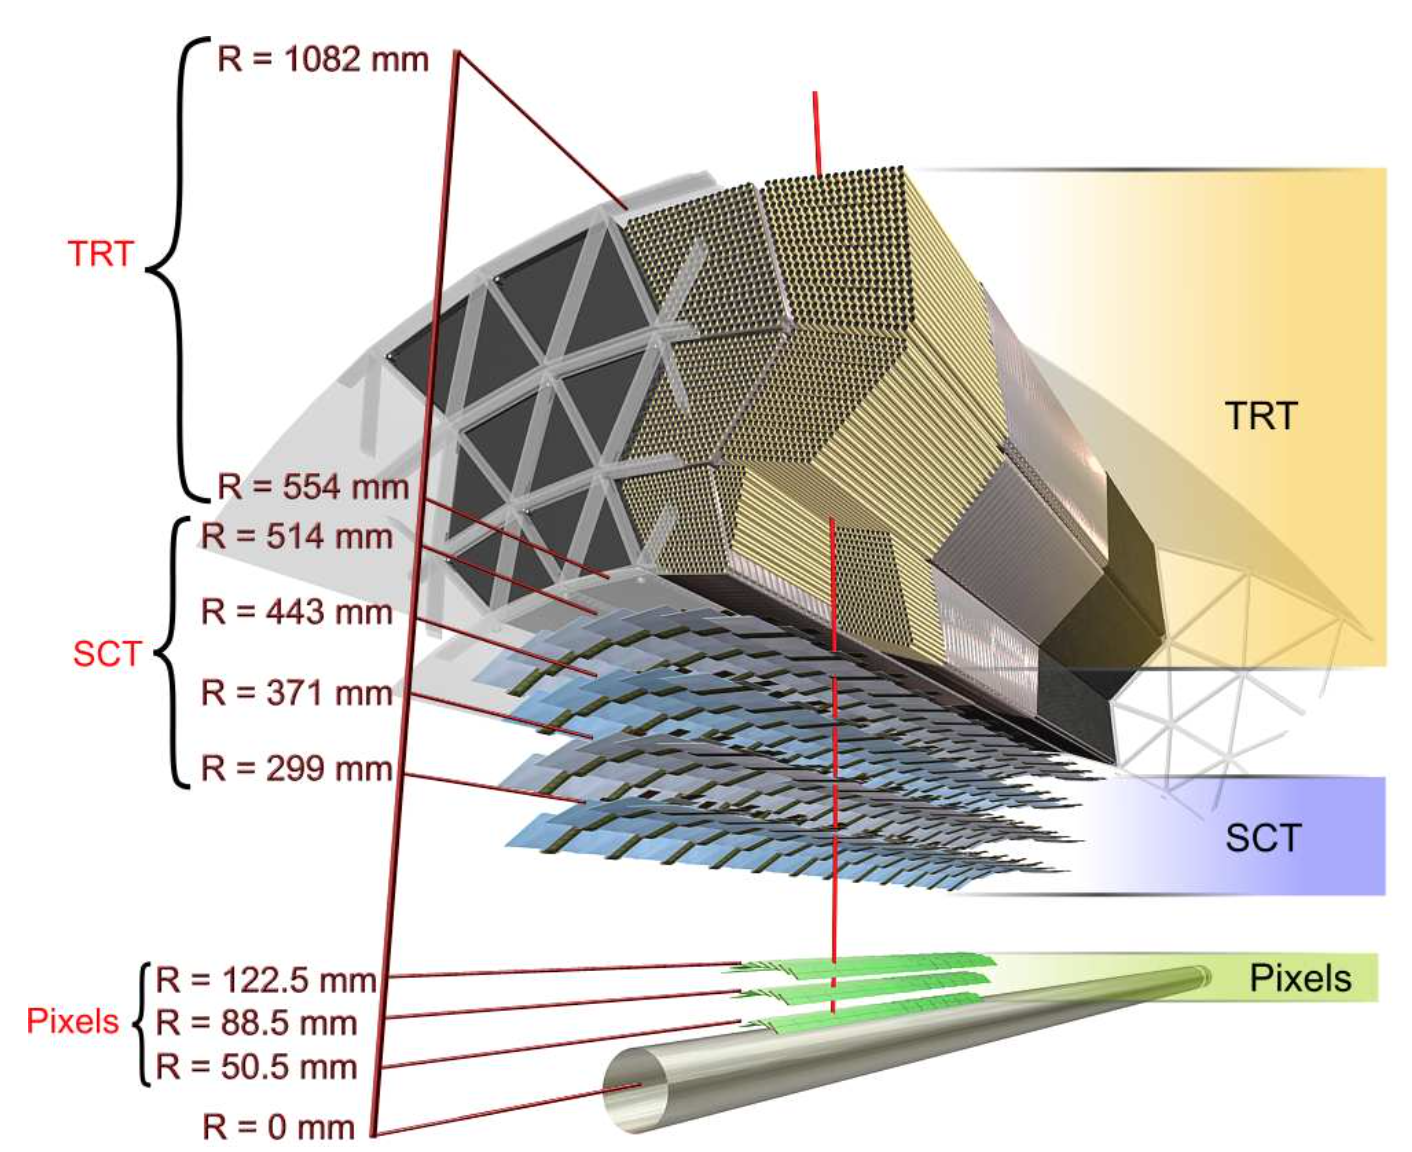
\includegraphics[width = \textwidth]{\figpath/ID_color.png}
\caption{The structural elements in the ID at $\eta = 0.3$~\cite{ATLAS_long}.}
\label{ID_color}
\end{figure}

\begin{figure}[h!tbp]
\centering
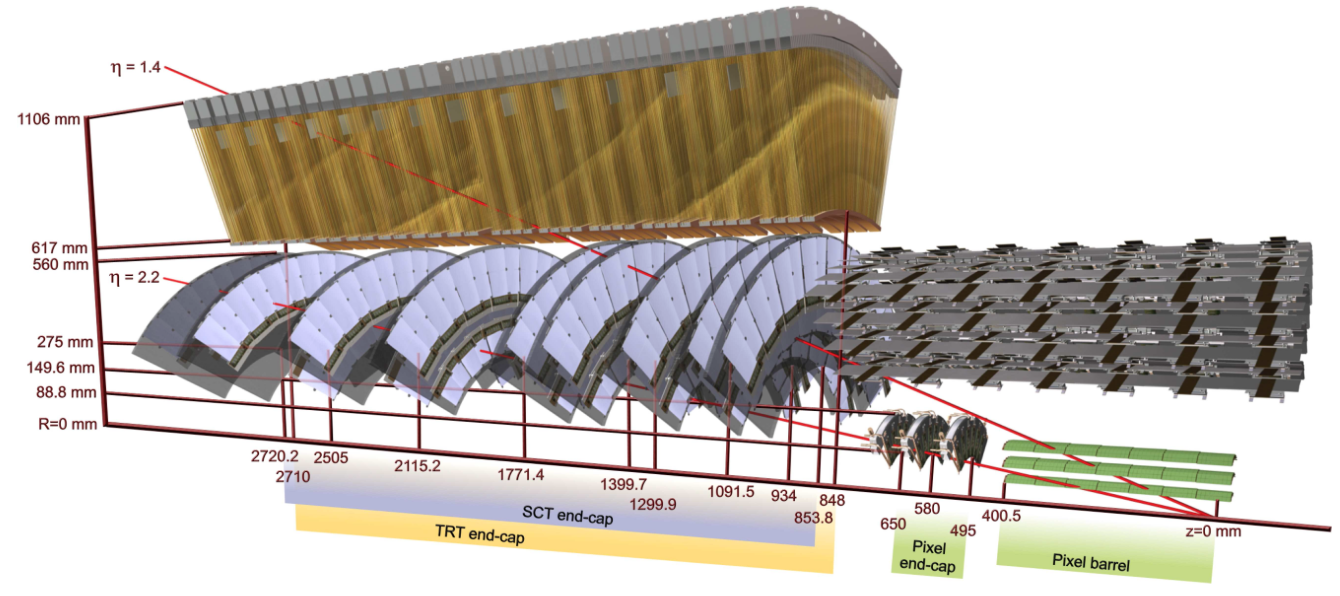
\includegraphics[width = \textwidth]{\figpath/ID_endcap.png}
\caption{The structural elements in the ID at $\eta = 1.4$~\cite{ATLAS_long}.}
\label{ID_endcap}
\end{figure}

\clearpage
\begin{wrapfigure}{r}{0.45\textwidth}
\centering
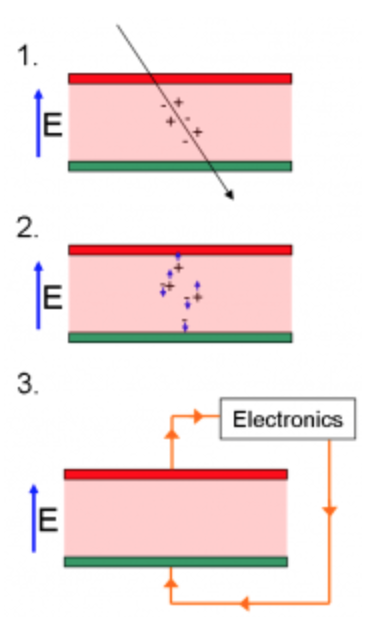
\includegraphics[width=0.4\textwidth]{\figpath/Pixel_cartoon.png}
\caption{Schematic for the general idea for how a pixel detector tracks incident particles.
~\cite{Quantum_diaries}}
\label{Pixel-cartoon}
\end{wrapfigure}

\subsubsection{Pixel Tracking System}

ATLAS is often referred to as a ``giant camera.''  
In a general sense, both a camera and the ATLAS detector provide ways to record specific events, but the parallels run deeper than their purposes, since both cameras and particle detectors can obtain information via pixels.  In a camera, an incident photon will go through a silicon diode and knock a valence electron free to generate a few electron-hole pairs.  An electric field is set up across the pixel and will then pull the electron and hole apart to the metal contacts where the charge can be read out \cite{Quantum_diaries}.  The pixel detector at ATLAS works in a similar way, except the energy of the incident particles at ATLAS is orders of magnitude larger: while a photon of visible light has an energy of a few eV, typical ``interesting'' particles at the LHC are in the MeV to TeV range.  

As a particle passes through the pixel sensor, it creates electron-hole pairs that are separated by the electric field and read out by the electronics, as shown in \Fig{Pixel-cartoon}. 

The pixel sensors in ATLAS consist of 80 million \cite{Detector_challenges} rectangular $50~\mu$m$ \times 400~\mu$m ``n$^+$-in-n'' electrodes.\footnote{The ``n'' region is n-type, or  doped with atoms that are electron donors; the ``in'' region is intrinsic, or undoped; and the ``n$^+$'' region is also n-type, but doped more heavily than other n region.}
The pixel detector's position with respect to the other components of the inner detector is shown in \Fig{ATLAS-InnerDetector}. 
Zooming in on  \Fig{ATLAS-InnerDetector}, the innermost part of the inner detector---the pixel detector---is shown in \Fig{ATLAS-PixelDetector}.  The 80 million channels are divided into four cylindrical layers combined in a volume 1442 mm in length with 430 mm radius \cite{Aad:2008Jinst}. The pixel detector has a resolution of 15 microns, and this precision is limited by the size of the electronics.

\begin{figure}[h!tbp]
\centering
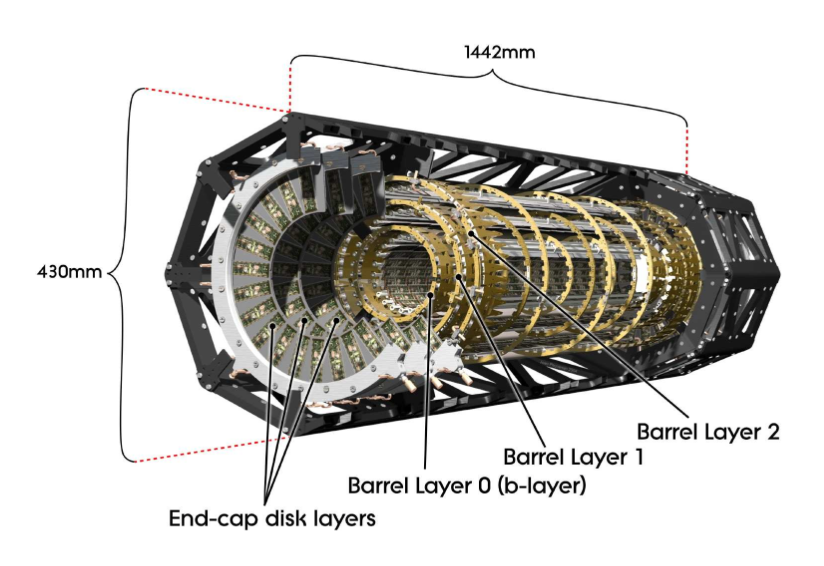
\includegraphics[scale=0.9]{\figpath/ATLAS_pixel_detector.png}
\caption{Illustration of the active region of the pixel detector with the barrel and endcap layers~\cite{Aad:2008Jinst}}
\label{ATLAS-PixelDetector}
\end{figure}

The pixel detector starts 5~cm from the center of the beam pipe to gain as much information about the central reaction as possible, and has coverage for $|\eta| < 2.5$~\cite{Detector_challenges}.
Since the pixel detector is so close to the interaction point, its electronics must be able to withstand high radiation doses of up to 500~kGy.  The p-n diodes can experience a leakage current when an electron-hole pair has enough energy to overcome the potential barrier.  
The detector minimizes the number of electron-hole pairs spontaneously generated by cooling the system at $-6^\circ$C.

\subsubsection{Silicon Microstrip Trackers}
The Silicon Microstrip Trackers (SCTs) operate with a similar principle as the pixel detectors, but have an effective operating voltage determined by the effective doping level, and their leakage current also increases linearly with radiation dose.
Initially the operating voltage was 150~V, but increased up to 250 to 350~V to compensate for the radiation dose after 10~years.
The 15912 SCT sensors each have a thickness of $285\pm15~\mu$m and a pitch of $80~\mu$m.
%(See p58 of ATLAS long for more details)

\subsubsection{Transition Radiation Tracker}
\label{trt}

The Transition Radiation Trackers (TRT) make up the outermost region of the ID, and the dimensions of the TRT are shown in \Fig{ID-table}.  ``Transition Radiation'' is the radiation emitted by a relativistic particle as it traverses an interface between two materials with different permittivities.
Each TRT is a 4~mm polyimide drift tube, created by two 35~$\mu$m multi-layer films bonded back-to-back \cite{ATLAS_long}.  
A 25~$\mu$m thick polyimide film has one side laminated with a 0.2 $\mu$m of Al with another 5-6~$\mu$m layer of graphite \cite{ATLAS_long}. 
The inside of the tube is filled with a gas composed of 70\%~Xe, 27\%~CO$_2$, and 3\%~O$_2$. 
The anode is composed of 31~$\mu$m diameter cylinder of tungsten wire positioned at the center of the drift tube, and coated with 0.5--0.7~$\mu$m of gold.
After fabrication, the tubes were cut to a 144~cm length for the barrel and 37~cm length for the end-cap region.  
The barrel straws are read out at each end of the tube, so the middle of the tube is insulated with a 6~mm glass layer which creates a 2~cm spot where the element is not sensitive to incident tracks.
The anode is grounded and connected to the front end electronics, while the cathodes are held at $-1530$V.  Minimizing mechanical sag in the straw is crucial for accounting for the error in the position measurements, so the straws are mechanically supported by carbon fibers \cite{ATLAS_long}.

\begin{figure}[h!tbp]
\centering
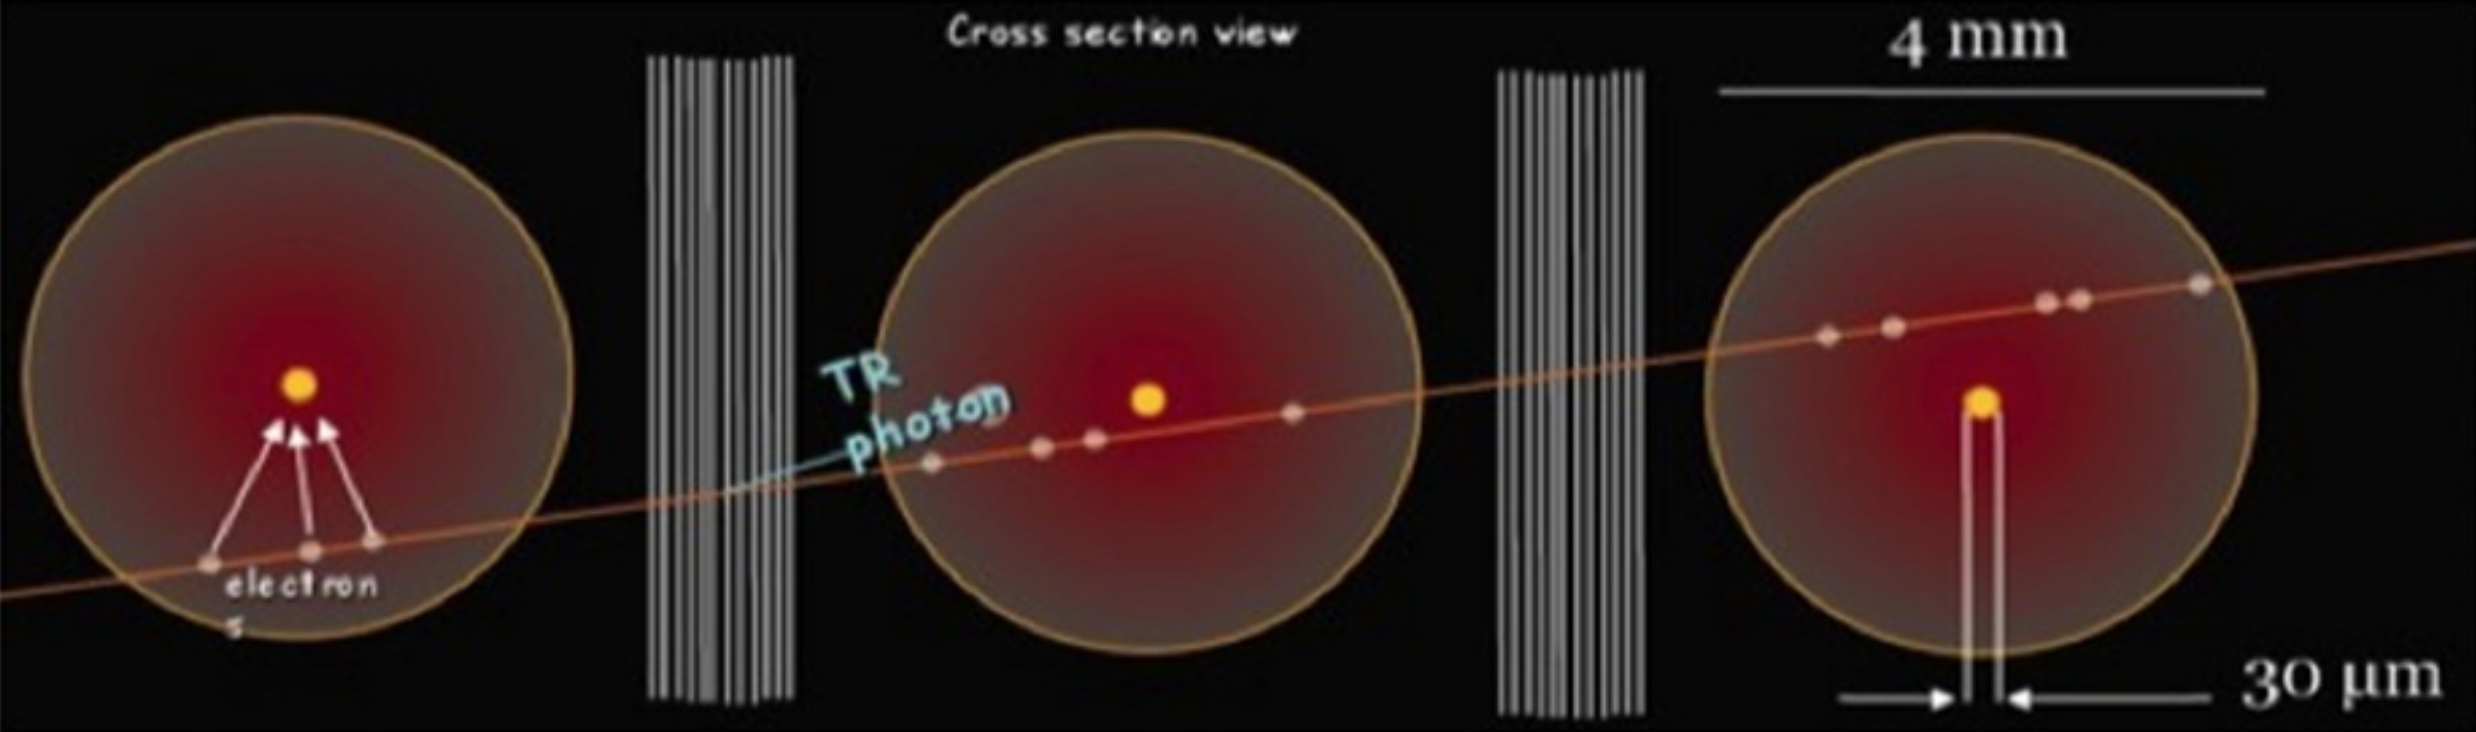
\includegraphics[width=\textwidth]{\figpath/TRT_cartoon.png}
\caption{Principle of operation for the TRT~\cite{TRT}}
\label{GEANT_sim}
\end{figure}

An incident particle traversing a straw ionizes the gas molecules to free electrons and positive ions.  The electrons accelerate through the electric field to the anode, and these electrons in turn will ionize other ions to create a gain of $2.5\times10^4$.  Since the anode is read out at both ends of the wire, this provides a drift time measurement from the difference of arrival times between the two ends of the wire.  The time resolution is approximately a nanosecond, which corresponds to a spatial resolution of about 100~microns.  

An outgoing particle will hit on average 36 of the TRT tubes; this improves the momentum measurement in the inner detector.
During its lifetime, a straw detector can track $10^{15}$ particles, and a total integrated charge of 1000~C, which corresponds to about 20~years of the LHC's operation.  
The ATLAS inner detector has 12,000 of these straws in the endcaps and 52,544 straws in the barrel, yielding a total of 351,000 read--out channels.  Although the silicon trackers need to be cooled between $-5$ to $-10^\circ$C, the TRTs operate at room temperature.

